\documentclass[12pt]{article}
\usepackage[utf8]{inputenc}
\usepackage{amsmath,amssymb,amsthm}
\usepackage{graphicx}
\usepackage{hyperref}
\usepackage{geometry}
\usepackage{tikz}
\usepackage{pgfplots}
\pgfplotsset{compat=1.17}
\usepackage{caption}
\usepackage{hyperref}

\title{FM3817B Assignment 1}
\author{Patrick Connors \\ Student Number: 251313609}
\date{\today}

\begin{document}

\maketitle

\section*{General Information}
\begin{itemize}
    \item \textbf{Created by:} Yifan Li
    \item \textbf{Due Date:} January 28, 2025, 11:55 pm
\end{itemize}

\subsection*{Instructions (Excerpted)}
\begin{itemize}
    \item Questions with bonus points: If you do it correctly, you will get the bonus points (until reaching full scores). Otherwise, no deduction. So feel free to try them out.
    \item More questions may be added progressively; the assignment will be finalized by January 21, 2025.
    \item You must submit a single PDF file through Gradescope. Format your submission carefully, assigning pages to corresponding questions.
    \item Late submissions are \textbf{not} accepted.
    \item You may discuss with classmates, but you must write and submit your own work. Scholastic offences are taken seriously.
\end{itemize}

\section*{Question 1 (6 pts)}
\textbf{Prospect Theory Utility Function.} Consider the utility function:
\[
U(x) = 
\begin{cases} 
x^\alpha, & \text{if } x \ge 0,\\
-\lambda \,(-x)^\alpha, & \text{if } x < 0,
\end{cases}
\]
where \(x\) represents gain or loss, and the parameters are set as \(\alpha = 0.9\) and \(\lambda = 2\).

\noindent \textbf{(a) First Derivative and Monotonicity}

\[
U(x) = 
\begin{cases}
x^\alpha, & x \ge 0,\\
-\lambda\,(-x)^\alpha, & x < 0.
\end{cases}
\]
\[
\alpha = 0.9, \quad \lambda = 2.
\]

\paragraph{Case 1: \(x>0\).} 
\[
U(x) = x^\alpha 
\quad \Longrightarrow \quad
U'(x) = \frac{d}{dx}\bigl(x^\alpha\bigr) = \alpha\, x^{\alpha - 1}.
\]
Since \(\alpha = 0.9\) and \(x>0\), we have \(x^{\alpha-1} = x^{-0.1} > 0\). Thus
\[
U'(x) = 0.9\, x^{-0.1} > 0,\quad \text{so }U(x)\text{ is increasing on }(0,\infty).
\]

\paragraph{Case 2: \(x<0\).} 
\[
U(x) = -\lambda\,(-x)^\alpha
\quad \Longrightarrow \quad
U'(x) = -\lambda \,\frac{d}{dx}\bigl[(-x)^\alpha\bigr].
\]
Since \(\frac{d}{dx}(-x)^\alpha = \alpha\,(-x)^{\alpha-1}\, \frac{d}{dx}(-x) = \alpha\,(-x)^{\alpha-1} \,(-1)\),
\[
U'(x) 
= -\lambda \,\Bigl[\alpha\,(-x)^{\alpha-1}\,(-1)\Bigr]
= \lambda\,\alpha\,(-x)^{\alpha-1}, \quad x<0.
\]
For \(x<0\), \(-x>0\), so \((-x)^{\alpha-1} >0\). Hence
\[
U'(x) = 2 \times 0.9 \times (-x)^{-0.1} = 1.8\,(-x)^{-0.1} >0,
\]
which means \(U(x)\) is also increasing on \((-\infty,0)\).

\newpage

\noindent \textbf{(b) Second Derivative and Convexity/Concavity}

\paragraph{Case 1: \(x>0\).} 
Starting from \(U'(x) = \alpha\, x^{\alpha-1}\):
\[
U''(x) = \alpha \,\frac{d}{dx}\bigl(x^{\alpha - 1}\bigr) 
= \alpha\,(\alpha - 1)\,x^{\alpha - 2}.
\]
With \(\alpha=0.9\), we have \(\alpha - 1 = -0.1\), so
\[
U''(x) = 0.9 \times (-0.1)\, x^{-1.1}
= -0.09\, x^{-1.1}, \quad x>0.
\]
Because \(x^{-1.1}>0\), \(U''(x)<0\). Hence \(U\) is \emph{concave} for \(x>0\).

\paragraph{Case 2: \(x<0\).} 
Starting from \(U'(x) = \lambda \,\alpha\,(-x)^{\alpha - 1}\):
\[
U''(x) 
= \lambda\,\alpha \,\frac{d}{dx}\bigl[(-x)^{\alpha-1}\bigr].
\]
Again, 
\[
\frac{d}{dx}\bigl[(-x)^{\alpha-1}\bigr]
= (\alpha-1)\,(-x)^{\alpha-2}\,\frac{d}{dx}(-x) 
= (\alpha-1)\,(-x)^{\alpha-2}\,(-1).
\]
Thus
\[
U''(x) 
= \lambda\,\alpha\, (\alpha-1)\,(-x)^{\alpha-2} \times (-1)
= -\,\lambda\,\alpha\,(\alpha-1)\,(-x)^{\alpha-2}, \quad x<0.
\]
Plug in \(\alpha=0.9,\;\lambda=2\). Then \(\alpha-1=-0.1\), so
\[
U''(x) 
= -\,2 \times 0.9 \times (-0.1)\,(-x)^{-1.1}
= 2 \times 0.9 \times 0.1 \,(-x)^{-1.1}
= 0.18\,(-x)^{-1.1}.
\]
That is \(>0\) for all \(x<0\). Hence \(U\) is \emph{convex} on \((-\infty,0)\).

\bigskip
\newpage

\noindent \textbf{(c) Continuity and Differentiability at \(x=0\)}

\paragraph{Continuity at \(x=0\).}
\[
\lim_{x \to 0^+}U(x) = \lim_{x\to 0^+} x^\alpha = 0,\qquad
\lim_{x \to 0^-}U(x) = \lim_{x\to 0^-} -\lambda\,(-x)^\alpha = -\,2\times 0 = 0,
\]
and \(U(0)\) can be taken as \(0^\alpha = 0\). Both one-sided limits agree with the value at 0, so \(\,U\) is \emph{continuous} at \(x=0\).  
\(\boxed{\text{Yes, it is continuous at } x=0.}\)

\paragraph{Differentiability at \(x=0\).}
Consider the \emph{right-hand} derivative:
\[
U'(0^+) = \lim_{x\to 0^+} \alpha\,x^{\alpha-1} 
= 0.9 \,\lim_{x\to 0^+} x^{-0.1} 
= +\infty.
\]
The \emph{left-hand} derivative:
\[
U'(0^-) 
= \lim_{x\to 0^-} \lambda\,\alpha\,(-x)^{\alpha-1}
= 1.8 \,\lim_{x\to 0^-} (-x)^{-0.1}
= +\infty.
\]
Neither side yields a finite derivative. Thus the function does \emph{not} have a well-defined (finite) slope at \(x=0\).  
\(\boxed{\text{No, it is not differentiable at }x=0.}\)

\begin{figure}[htbp]
    \centering
    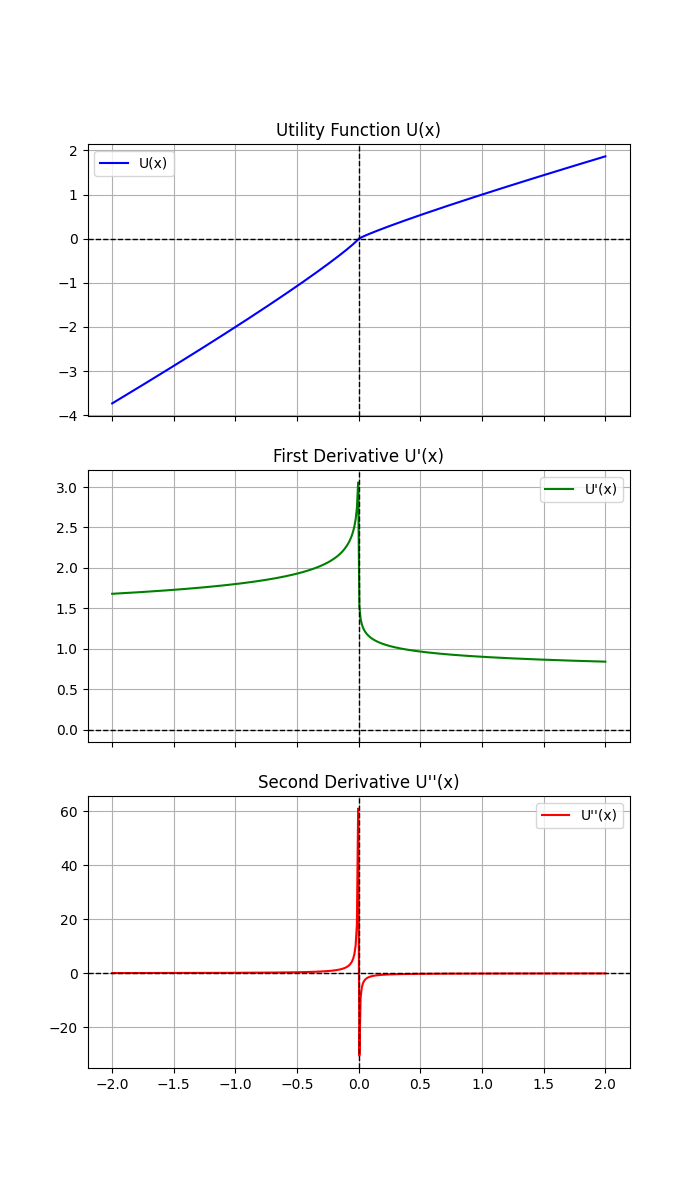
\includegraphics[width=0.7\textwidth]{q1.png}
    \caption{Graphs of \(U(x)\) and its first two derivatives.}
    \label{fig:my_label}
\end{figure}

\newpage

\section*{Question 2 (12 pts)}
\textbf{Set Analysis.} Consider the set \(S = [1, 2) \cup (2, 3]\). Answer the following:

\subsection*{Answer:}

\noindent \textbf{(a) Is \(S\) a closed set? (Yes or No) Why?}

\[
S \;=\; [1,2) \;\cup\; (2,3]
\]
is \textbf{not} closed.

\paragraph{Explanation:}

We use the given definition of a closed set:

\begin{quote}
A set \( S \subset \mathbb{R} \) is closed if and only if for \textit{every} convergent sequence \( \{x_n\} \subset S \), the limit of that sequence also lies in \( S \).
\end{quote}

To show that \( S \) is \textit{not} closed, it suffices to exhibit \textbf{one} convergent sequence entirely contained in \( S \) whose limit does \textit{not} belong to \( S \).

\paragraph{Detailed Steps:}

\begin{enumerate}
    \item Observe that \( S \) is the union of the two intervals:
    \[
    [1,2) \quad \text{and} \quad (2,3].
    \]
    Notice that the number \( 2 \) is \textit{excluded} from both intervals:
    \[
    2 \notin [1,2) 
    \quad \text{and} \quad 
    2 \notin (2,3].
    \]
    Hence, \( 2 \notin S \).
    
    \item Consider the sequence \( \{x_n\} \) defined by  
    \[
    x_n \;=\; 2 - \tfrac{1}{n} \quad (n = 1, 2, 3, \dots).
    \]
    
    \item \textbf{Check that \( x_n \) lies in \( S \) for all \( n \):}  
    \begin{itemize}
        \item For each \( n \),
        \[
        2 - \tfrac{1}{n} < 2,
        \]
        which means \( x_n < 2 \).
        
        \item Also, \( 2 - \tfrac{1}{n} \geq 1 \) for all \( n \geq 1 \).
        
        \item Therefore,
        \[
        1 \;\leq\; 2 - \tfrac{1}{n} \;<\; 2,
        \]
        so \( x_n \in [1,2) \). Since \( [1,2) \subset S \), we have \( x_n \in S \) for \textit{every} \( n \).
    \end{itemize}
    
    \item \textbf{Determine the limit of \( \{x_n\} \)}:  
    \[
    \lim_{n \to \infty} \Bigl(2 - \tfrac{1}{n}\Bigr) \;=\; 2.
    \]
    
    \item \textbf{Check if the limit \( 2 \) belongs to \( S \)}:  
    \begin{itemize}
        \item We already noted that \( 2 \notin S \).
    \end{itemize}
\end{enumerate}

Thus, we have constructed a sequence \( \{x_n\} \subset S \) which converges to a point (\( 2 \)) \textit{outside} of \( S \).

\bigskip

\noindent \textbf{Conclusion}

Because there exists at least one sequence \( \{x_n\} \subset S \) converging to a limit that is not in \( S \), \( S \) fails the criterion for being a closed set. Therefore,

\[
\boxed{ S \text{ is not closed.} }
\]
\newpage

\noindent \textbf{(b.) Is $S$ an open set? (Yes or No) Why? (Please state two different pieces of evidence for this question.)}

No, the set $S = [1, 2) \cup (2, 3]$ is not an open set. To determine this, we use the formal definition of an open set: a set $S \subseteq \mathbb{R}$ is open if, for every point $x \in S$, there exists an $\epsilon > 0$ such that the open interval $(x - \epsilon, x + \epsilon) \subseteq S$. Two specific pieces of evidence are:

\begin{itemize}
    \item Consider the point $x = 1$. The point $x = 1$ belongs to $S$ because it is part of the interval $[1, 2)$. However, for any $\epsilon > 0$, the interval $(1 - \epsilon, 1)$ will include points less than $1$, which are not in $S$. Therefore, no suitable $\epsilon$ exists, and $S$ is not open at $x = 1$.
    
    \item Consider the point $x = 3$. The point $x = 3$ belongs to $S$ because it is part of the interval $(2, 3]$. However, for any $\epsilon > 0$, the interval $(3, 3 + \epsilon)$ will include points greater than $3$, which are not in $S$. Hence, no suitable $\epsilon$ exists, and $S$ is not open at $x = 3$.
\end{itemize}

\noindent Since there exist points in $S$ where the condition for openness is not satisfied, the set $S$ is \textbf{not open}.

\bigskip
\newpage
\subsection*{(c) Is \(S\) a convex set?}

\noindent Recall the set:
\[
S = [1, 2) \cup (2, 3].
\]

\paragraph{Answer:} No, \(S\) is not convex.

\paragraph{Reason:}

A set \(S \subseteq \mathbb{R}\) is \textbf{convex} if and only if, for \textbf{every} pair of points \(x, y \in S\), the entire line segment
\[
\{ tx + (1-t)y : t \in [0,1] \}
\]
is contained in \(S\).

\begin{enumerate}
    \item Observe that \(2 \notin S\). Indeed:
    \begin{itemize}
        \item \(2\) is not in \([1,2)\) because that interval excludes the endpoint \(2\).
        \item \(2\) is not in \((2,3]\) because that interval excludes \(2\).
    \end{itemize}
    \item To see the lack of convexity, pick one point \textit{on each side} of the gap. For instance:
    \[
    x = 1.5 \in [1,2), \quad y = 2.5 \in (2,3].
    \]
    \item Consider the midpoint (i.e., \(t = \frac{1}{2}\)) on the line segment between \(x\) and \(y\):
    \[
    \frac{1}{2}x + \frac{1}{2}y = \frac{1}{2}(1.5) + \frac{1}{2}(2.5) = 2.
    \]
    \item But \(2 \notin S\). Hence, the line segment between \(x\) and \(y\) is \textbf{not} fully contained in \(S\).
\end{enumerate}

Since we found two points in \(S\) whose connecting line segment is \textbf{not} contained in \(S\), this violates the definition of convexity. Therefore, \(S\) is \textbf{not} a convex set.

\bigskip
\newpage
\subsection*{(d) Modifying \(S\) to make it convex}

Since the only problem with \(S\) is the missing point at \(x = 2\), the \textbf{simplest} fix is to \textbf{include} that point. In fact, if you fill that gap, you end up with the entire interval from \(1\) to \(3\).

\paragraph{Answer:} A natural choice is
\[
S^* = [1, 3].
\]
Equivalently, one could write \(S^*\) as \([1,2] \cup (2,3]\), which simplifies to the same interval \([1,3]\). Either form will be a convex set in \(\mathbb{R}\).

\bigskip
\newpage
\subsection*{(e) Proving that \(S^*\) is convex}

Let us use the definition of convexity for \(S^*\). We will show that for \textbf{any} \(x, y \in S^*\) and \textbf{any} \(t \in [0,1]\), the point
\[
z = t x + (1 - t) y
\]
is also in \(S^*\).

\begin{enumerate}
    \item We have \(S^* = [1,3]\).
    \item If \(x, y \in [1,3]\), then \(1 \le x \le 3\) and \(1 \le y \le 3\).
    \item For any \(t \in [0,1]\), the point \(z = t x + (1-t) y\) must lie \textbf{between} \(x\) and \(y\). Concretely,
    \[
    \min(x,y) \le t x + (1-t) y \le \max(x,y).
    \]
    \item Since \(\min(x,y) \ge 1\) and \(\max(x,y) \le 3\), it follows that
    \[
    1 \le z \le 3.
    \]
    \item Therefore, \(z \in [1,3]\). Hence \(z \in S^*\).
\end{enumerate}

Since \(z\) remains in \(S^*\) for \textbf{every} choice of \(x, y \in S^*\) and \(t \in [0,1]\), \(S^*\) is \textbf{convex} by definition.

\bigskip
\newpage
\section*{Question 3 (12 pts)}

Consider the function \( f : [-8, 5] \to \mathbb{R} \), defined by
\[
f(x) = 2x^3 + 3x^2 - 72x + 40.
\]

\subsection*{(a) Interior and Boundary Points}

\begin{enumerate}
    \item \textbf{Boundary Points} \\
    The boundary points of the interval \([-8, 5]\) are its endpoints:
    \[
    \boxed{x = -8 \quad \text{and} \quad x = 5}.
    \]
    
    \item \textbf{Interior Points} \\
    All points strictly between \(-8\) and \(5\) form the interior:
    \[
    \boxed{\text{Interior} = (-8, 5)}.
    \]
\end{enumerate}
\newpage
\subsection*{(b) Compute all critical points of \( f(x) \)}


A critical point \(x\) of \(f\) occurs where the derivative \(f'(x)\) is zero or undefined. Since \(f(x)\) is a polynomial (which is differentiable everywhere), we only need to solve \(f'(x) = 0\).

\paragraph{Step 1: Compute the derivative}

\[
\begin{aligned}
f(x) &= 2x^3 + 3x^2 - 72x + 40,\\[6pt]
f'(x) &= \frac{d}{dx}\bigl(2x^3\bigr) 
      + \frac{d}{dx}\bigl(3x^2\bigr) 
      - \frac{d}{dx}\bigl(72x\bigr) 
      + \frac{d}{dx}\bigl(40\bigr).
\end{aligned}
\]

Calculating each term:
\begin{align*}
\frac{d}{dx}\bigl(2x^3\bigr) &= 6x^2, \\
\frac{d}{dx}\bigl(3x^2\bigr) &= 6x, \\
\frac{d}{dx}\bigl(72x\bigr) &= 72, \\
\frac{d}{dx}\bigl(40\bigr) &= 0.
\end{align*}

Thus,
\[
\boxed{
f'(x) = 6x^2 + 6x - 72.
}
\]

\paragraph{Step 2: Solve \(f'(x) = 0\)}

Set the derivative equal to zero:
\[
6x^2 + 6x - 72 = 0.
\]

Simplify by dividing by 6:
\[
x^2 + x - 12 = 0.
\]

Factor the quadratic equation:
\[
x^2 + x - 12 = (x - 3)(x + 4) = 0.
\]

Therefore,
\[
\boxed{x = 3 \quad \text{or} \quad x = -4}.
\]

Both \(x = -4\) and \(x = 3\) lie within the interval \([-8, 5]\), so they are critical points of \(f\).
\newpage
\subsection*{(c) Determine all local maxima and minima of \( f(x) \)}


To classify the critical points \(x = -4\) and \(x = 3\) as local maxima or minima, we use the Second Derivative Test.

\paragraph{Step: Compute the second derivative \(f''(x)\)}

Starting from \(f'(x) = 6x^2 + 6x - 72\),
\[
\boxed{
f''(x) = \frac{d}{dx}(6x^2) + \frac{d}{dx}(6x) - \frac{d}{dx}(72) 
        = 12x + 6.
}
\]

\paragraph{Classify Each Critical Point}

\begin{enumerate}
    \item \textbf{At \(x = -4\):}  
    \[
    f''(-4) = 12(-4) + 6 = -48 + 6 = -42 < 0.
    \]
    Since \(f''(-4) < 0\), the function is concave down at \(x = -4\). Therefore,
    \[
    \boxed{x = -4 \text{ is a local maximum.}}
    \]
    
    \item \textbf{At \(x = 3\):}  
    \[
    f''(3) = 12(3) + 6 = 36 + 6 = 42 > 0.
    \]
    Since \(f''(3) > 0\), the function is concave up at \(x = 3\). Therefore,
    \[
    \boxed{x = 3 \text{ is a local minimum.}}
    \]
\end{enumerate}
\newpage
\subsection*{(d) Find the global maximum and minimum values of \( f(x) \) on \([-8, 5]\)}

A global maximum or minimum over a closed interval \([a, b]\) occurs either at a critical point in \((a, b)\) or at an endpoint of the interval.

\paragraph{Step 1: Evaluate \(f\) at all critical points}

\begin{enumerate}
    \item \(f(-4)\):
    \[
    \begin{aligned}
    f(-4) &= 2(-4)^3 + 3(-4)^2 - 72(-4) + 40 \\[4pt]
           &= 2(-64) + 3(16) + 288 + 40 \\[4pt]
           &= -128 + 48 + 288 + 40 \\[4pt]
           &= (-128 + 48) + 288 + 40 \\[4pt]
           &= -80 + 288 + 40 \\[4pt]
           &= 208 + 40 \\[4pt]
           &= 248.\\[4pt]
    \boxed{f(-4) = 248.}
    \end{aligned}
    \]
    
    \item \(f(3)\):
    \[
    \begin{aligned}
    f(3) &= 2(3)^3 + 3(3)^2 - 72(3) + 40 \\[4pt]
          &= 2(27) + 3(9) - 216 + 40 \\[4pt]
          &= 54 + 27 - 216 + 40 \\[4pt]
          &= 81 - 216 + 40 \\[4pt]
          &= -135 + 40 \\[4pt]
          &= -95. \\[4pt]
    \boxed{f(3) = -95.}
    \end{aligned}
    \]
\end{enumerate}

\paragraph{Step 2: Evaluate \(f\) at the endpoints}

\begin{enumerate}
    \item \(f(-8)\):
    \[
    \begin{aligned}
    f(-8) &= 2(-8)^3 + 3(-8)^2 - 72(-8) + 40 \\[4pt]
          &= 2(-512) + 3(64) + 576 + 40 \\[4pt]
          &= -1024 + 192 + 576 + 40 \\[4pt]
          &= -1024 + (192 + 576) + 40 \\[4pt]
          &= -1024 + 768 + 40 \\[4pt]
          &= -256 + 40 \\[4pt]
          &= -216.\\[4pt]
    \boxed{f(-8) = -216.}
    \end{aligned}
    \]
    
    \item \(f(5)\):
    \[
    \begin{aligned}
    f(5) &= 2(5)^3 + 3(5)^2 - 72(5) + 40 \\[4pt]
         &= 2(125) + 3(25) - 360 + 40 \\[4pt]
         &= 250 + 75 - 360 + 40 \\[4pt]
         &= 325 - 360 + 40 \\[4pt]
         &= -35 + 40 \\[4pt]
         &= 5.\\[4pt]
    \boxed{f(5) = 5.}
    \end{aligned}
    \]
\end{enumerate}

\paragraph{Step 3: Determine the global maximum and minimum}

We have the following function values:
\[
\begin{aligned}
& f(-8) = -216,\\
& f(-4) = 248,\\
& f(3)  = -95,\\
& f(5)  = 5.
\end{aligned}
\]

\begin{itemize}
    \item \textbf{Global Maximum}: The largest of these values is \(248\), which occurs at \(x = -4\).
    \[
    \boxed{\text{Global Maximum} = 248 \text{ at } x = -4.}
    \]
    
    \item \textbf{Global Minimum}: The smallest of these values is \(-216\), which occurs at \(x = -8\).
    \[
    \boxed{\text{Global Minimum} = -216 \text{ at } x = -8.}
    \]
\end{itemize}
\newpage

\subsection*{(e) Sketch the Graph of \( f(x) \) over \([-8, 5]\)}

Below is a sketch of the graph highlighting the critical and boundary points, as well as the global extrema.

\begin{figure}[h!]
    \centering
    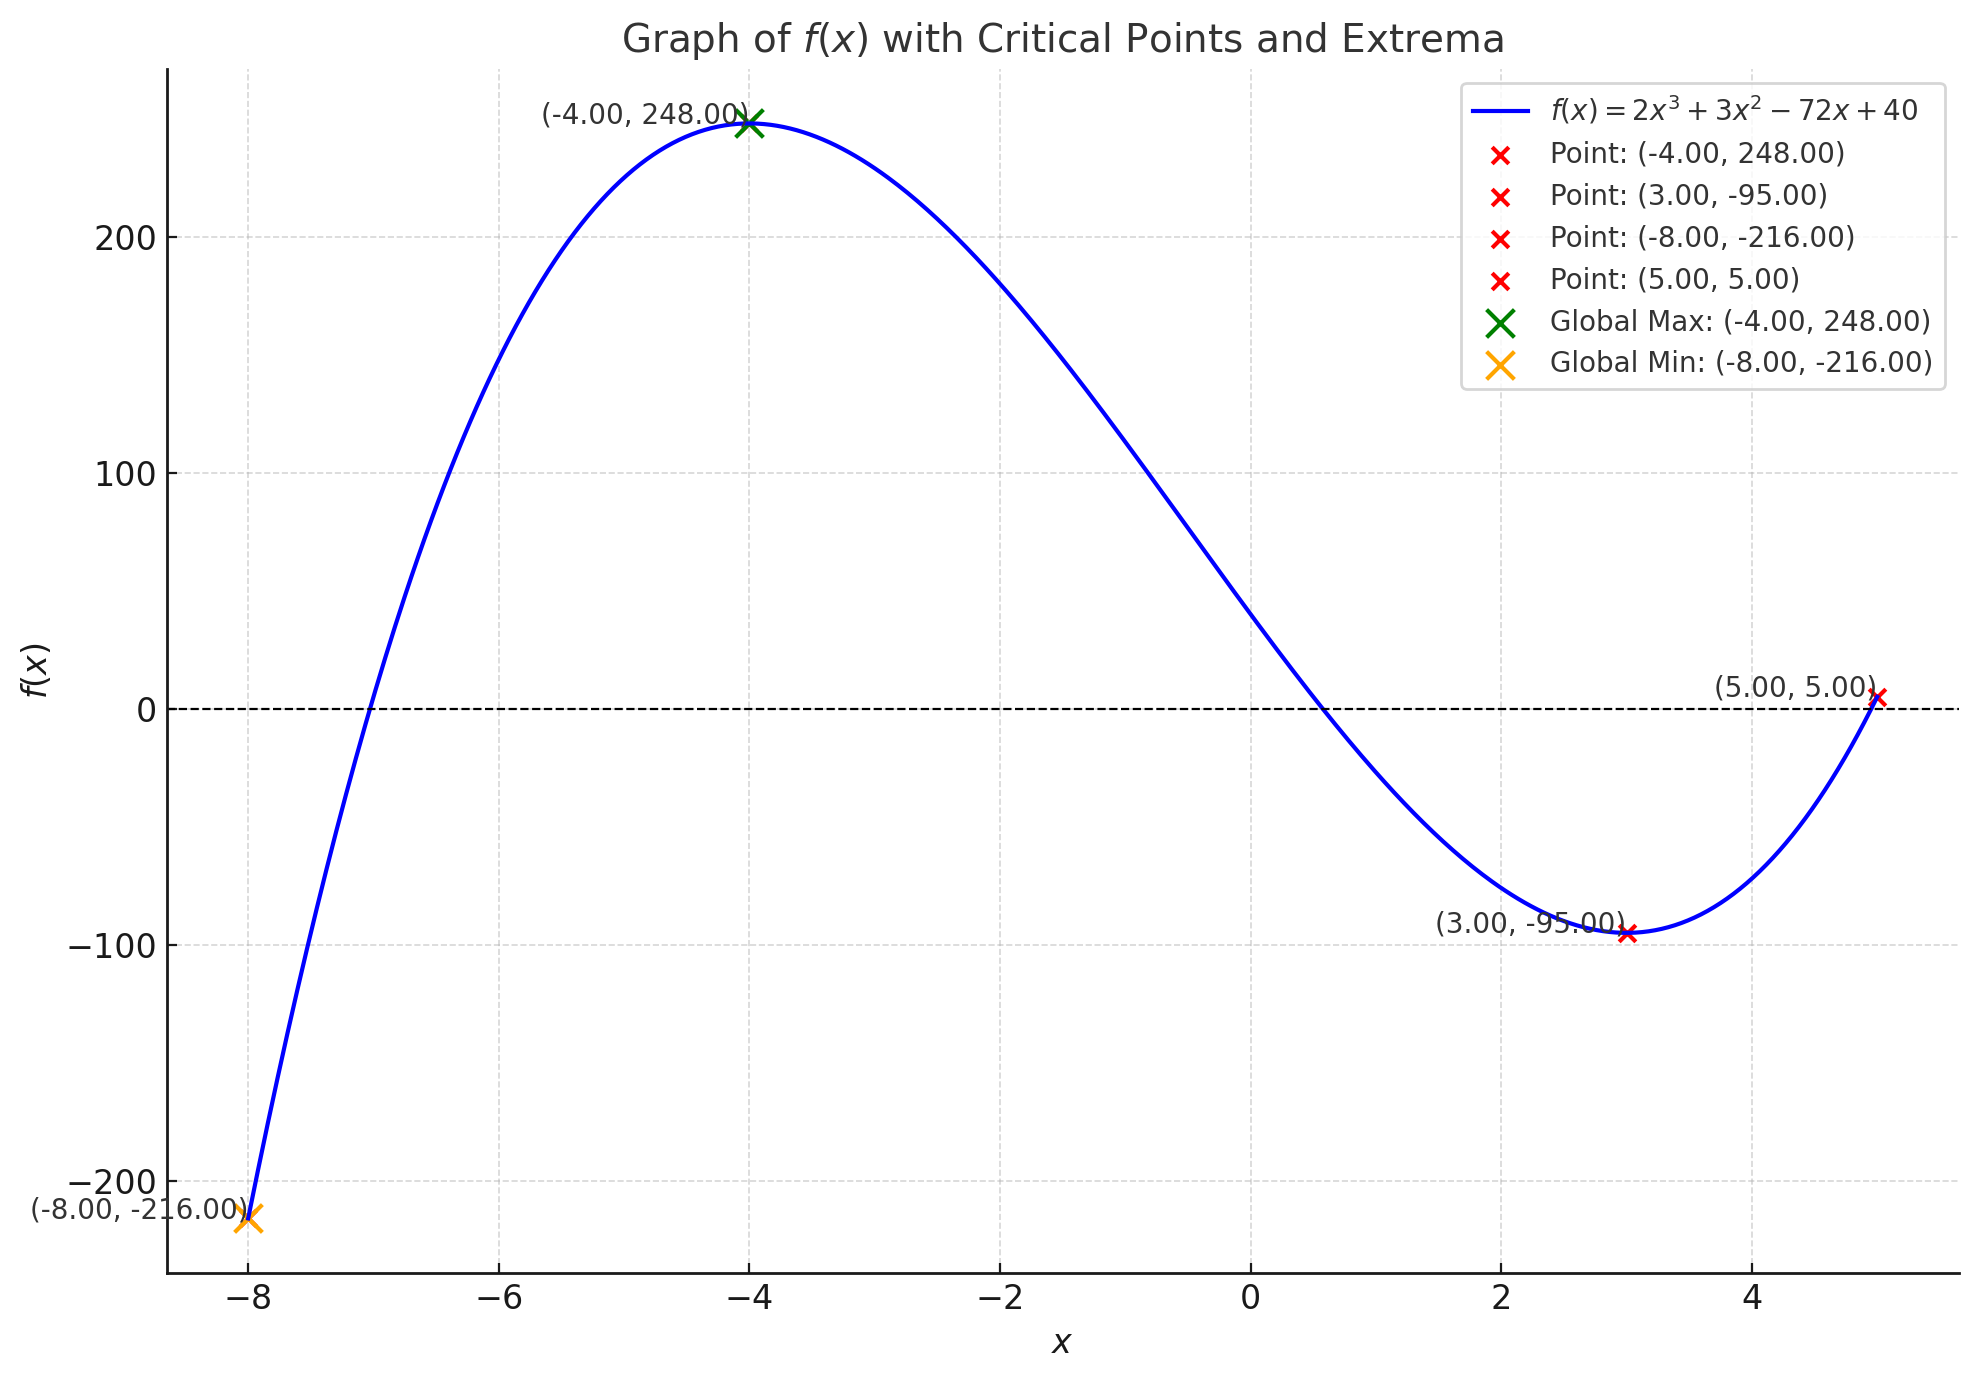
\includegraphics[width=0.8\textwidth]{q3.png} % Update the path if needed
    \caption{Graph of \( f(x) \) with critical points and extrema.}
    \label{fig:f_graph}
\end{figure}

\newpage

\section*{Question 4 (8 pts)}

For each of the following functions, find the critical point(s) and classify them as local max, local min, saddle point or inconclusive.

\subsection*{(a) \( f(x, y) = x^4 + x^2 - 6xy + 3y^2 \)}

\subsubsection*{Critical Points}
\begin{enumerate}
    \item \((-1.000, -1.000)\)
    \item \((0, 0)\)
    \item \((1.000, 1.000)\)
\end{enumerate}

\subsubsection*{Classification}
\begin{itemize}
    \item \textbf{Local minima:}
    \begin{itemize}
        \item \((-1.0000, -1.0000)\), \( f(x,y) = -1.0000 \)
        \item \((1.0000, 1.0000)\), \( f(x,y) = -1.0000 \)
    \end{itemize}
    \item \textbf{Local maxima:} None
    \item \textbf{Saddle points:}
    \begin{itemize}
        \item \((0.0000, 0.0000)\), \( f(x,y) = 0.0000 \)
    \end{itemize}
    \item \textbf{Inconclusive points:} None
\end{itemize}

\hrulefill
\newpage


\subsection*{(b) \( f(x, y) = x^2 - 6xy + 2y^2 + 10x + 2y - 5 \)}

\subsubsection*{Critical Points}
\begin{enumerate}
    \item \((1.857, 2.286)\)
\end{enumerate}

\subsubsection*{Classification}
\begin{itemize}
    \item \textbf{Local minima:} None
    \item \textbf{Local maxima:} None
    \item \textbf{Saddle points:}
    \begin{itemize}
        \item \((1.8571, 2.2857)\), \( f(x,y) = 6.5714 \)
    \end{itemize}
    \item \textbf{Inconclusive points:} None
\end{itemize}

\hrulefill
\newpage

\subsection*{(c) \( f(x, y) = xy^2 + x^3y - xy \)}

\subsubsection*{Critical Points}
\begin{enumerate}
    \item \((-1.000, 0)\)
    \item \((0, 0)\)
    \item \((0, 1.000)\)
    \item \((1.000, 0)\)
    \item \((-0.4472, 0.4000)\)
    \item \((0.4472, 0.4000)\)
\end{enumerate}

\subsubsection*{Classification}
\begin{itemize}
    \item \textbf{Local minima:}
    \begin{itemize}
        \item \((0.4472, 0.4000)\), \( f(x,y) = -0.0716 \)
    \end{itemize}
    \item \textbf{Local maxima:}
    \begin{itemize}
        \item \((-0.4472, 0.4000)\), \( f(x,y) = 0.0716 \)
    \end{itemize}
    \item \textbf{Saddle points:}
    \begin{itemize}
        \item \((-1.0000, 0.0000)\), \( f(x,y) = 0.0000 \)
        \item \((0.0000, 0.0000)\), \( f(x,y) = 0.0000 \)
        \item \((0.0000, 1.0000)\), \( f(x,y) = 0.0000 \)
        \item \((1.0000, 0.0000)\), \( f(x,y) = 0.0000 \)
    \end{itemize}
    \item \textbf{Inconclusive points:} None
\end{itemize}

\hrulefill
\newpage

\subsection*{(d) \( f(x, y) = 3x^4 + 3x^2y - y^3 \)}

\subsubsection*{Critical Points}
\begin{enumerate}
    \item \((-0.5000, -0.5000)\)
    \item \((0, 0)\)
    \item \((0.5000, -0.5000)\)
\end{enumerate}

\subsubsection*{Classification}
\begin{itemize}
    \item \textbf{Local minima:}
    \begin{itemize}
        \item \((-0.5000, -0.5000)\), \( f(x,y) = -0.0625 \)
        \item \((0.5000, -0.5000)\), \( f(x,y) = -0.0625 \)
    \end{itemize}
    \item \textbf{Local maxima:} None
    \item \textbf{Saddle points:} None
    \item \textbf{Inconclusive points:}
    \begin{itemize}
        \item \((0.0000, 0.0000)\), \( f(x,y) = 0.0000 \)
    \end{itemize}
\end{itemize}

\hrulefill
\newpage

\section*{Question 5 (8 pts)}

Below we determine which (if any) of the critical points found in Question 4 
are \emph{global} maxima or minima. 

\subsection*{(a) \texorpdfstring{$f(x, y) = x^4 + x^2 - 6xy + 3y^2$}{f(x, y) = x^4 + x^2 - 6xy + 3y^2}}

\begin{itemize}
    \item \textbf{Critical points found in Question 4:} 
          \[
             (0,0),\quad (1,1),\quad (-1,-1).
          \]
    \item \textbf{Local classification (from Hessian tests):}
    \begin{itemize}
        \item $(0,0)$ is a saddle point.
        \item $(1,1)$ and $(-1,-1)$ are local minima.
    \end{itemize}
    \item \textbf{Behavior at infinity:} 
    Since $x^4 \to +\infty$ as $\|x\|\to \infty$, the function $f(x,y)$ 
    also tends to $+\infty$ for large $|x|$. Hence, there is no global maximum.
    \item \textbf{Global minima:} 
    Both $(1,1)$ and $(-1,-1)$ give the same minimum value 
    \[
       f(\pm 1,\pm 1) \;=\; 1 + 1 - 6 \cdot 1 \cdot 1 + 3 = -1.
    \]
    Since $f \to +\infty$ elsewhere, these two points are \textbf{global minima}. 
\end{itemize}

\paragraph{Conclusion for (a):} 
\emph{The points $(1,1)$ and $(-1,-1)$ are global minima; there is no global maximum.}
\newpage
\subsection*{(b) \texorpdfstring{$f(x, y) = x^2 - 6xy + 2y^2 + 10x + 2y - 5$}{f(x, y) = x^2 - 6xy + 2y^2 + 10x + 2y - 5}}

\begin{itemize}
    \item \textbf{Critical point from Question 4:}
          \[
              \left(\frac{13}{7},\, \frac{16}{7}\right).
          \]
    \item \textbf{Local classification:} 
    The Hessian of this quadratic form is
    \[
        H = \begin{pmatrix} 2 & -6 \\ -6 & 4 \end{pmatrix},
    \]
    which has determinant $2\cdot 4 - (-6)\cdot(-6) = 8 - 36 = -28 < 0$. 
    Therefore the quadratic form is indefinite, and the critical point is a saddle.
    \item \textbf{Global behavior:} 
    Since the quadratic form is indefinite, the function $f$ can take arbitrarily 
    large positive and negative values by moving along certain directions in $\mathbb{R}^2$. 
    Hence there is \emph{no global maximum} and \emph{no global minimum}.
\end{itemize}

\paragraph{Conclusion for (b):}
\emph{There is no global maximum or minimum (the lone critical point is a saddle).}
\newpage
\subsection*{(c) \texorpdfstring{$f(x, y) = xy^2 + x^3y - xy$}{f(x, y) = xy^2 + x^3y - xy}}

\begin{itemize}
    \item \textbf{Critical points (from Question 4):} 
    \[
       (0,0),\quad (0,1),\quad (1,0),\quad (-1,0),\quad 
       \left(\tfrac{1}{\sqrt{5}},\, \tfrac{2}{5}\right),\quad
       \left(-\tfrac{1}{\sqrt{5}},\, \tfrac{2}{5}\right).
    \]
    \item \textbf{Global behavior:}
    Since $f(x,y)$ is a cubic polynomial, it is \emph{not bounded} above or below. 
    For large $|x|$ and $|y|$, the terms like $x^3y$ can dominate and make $f$ go to 
    $+\infty$ or $-\infty$ in suitable directions.
\end{itemize}

\paragraph{Conclusion for (c):} 
\emph{There are no global maxima or minima.}
\newpage
\subsection*{(d) \texorpdfstring{$f(x, y) = 3x^4 + 3x^2y - y^3$}{f(x, y) = 3x^4 + 3x^2y - y^3}}

\begin{itemize}
    \item \textbf{Critical points (from Question 4):}
    \[
       (0,0),\quad \left(\tfrac{1}{2}, -\tfrac{1}{2}\right),\quad \left(-\tfrac{1}{2}, -\tfrac{1}{2}\right).
    \]
    \item \textbf{Global behavior:} 
    As $|x|\to \infty$, the term $3x^4 \to +\infty$. 
    On the other hand, as $|y| \to \infty$ with $y>0$, the term $-y^3 \to -\infty$. 
    Hence $f$ is not bounded above or below. 
    Therefore there can be no global extrema.
\end{itemize}

\paragraph{Conclusion for (d):} 
\emph{No global maximum or minimum exists (the function is unbounded above and below).}

\vfill
\newpage
\textbf{Final Summary:}
\begin{itemize}
    \item For part (a): The only global minima are $(1,1)$ and $(-1,-1)$ (value = $-1$). No global max.
    \item For parts (b), (c), and (d): \emph{No global maxima or minima} exist.
\end{itemize}

\newpage

\section*{Question 6 (6 pts)}

In economics and finance, a famous class of utility functions is called the Cobb-Douglas utility function. Such a function is in the form 
\[
U(x, y) = kx^a y^b
\]
where \(a, b \in (0, 1)\) and \(k > 0\).

\subsection*{(a) Jacobian of \(U(x, y)\)}

\subsubsection*{1. Definition of the Jacobian}
The Jacobian matrix is the row vector of first-order partial derivatives:
\[
J_U(x, y) = \begin{bmatrix}
\frac{\partial U}{\partial x} & \frac{\partial U}{\partial y}
\end{bmatrix}.
\]

\subsubsection*{2. Compute the partial derivatives}
\[
\frac{\partial U}{\partial x} = k a x^{a-1} y^b, \quad \frac{\partial U}{\partial y} = k b x^a y^{b-1}.
\]

\subsubsection*{3. Result}
The Jacobian matrix is:
\[
J_U(x, y) = \begin{bmatrix}
k a x^{a-1} y^b & k b x^a y^{b-1}
\end{bmatrix}.
\]
\newpage
\subsection*{(b) Hessian of \(U(x, y)\)}

\subsubsection*{1. Definition of the Hessian}
The Hessian matrix is the matrix of second-order partial derivatives:
\[
H_U(x, y) = \begin{bmatrix}
\frac{\partial^2 U}{\partial x^2} & \frac{\partial^2 U}{\partial x \partial y} \\[8pt]
\frac{\partial^2 U}{\partial y \partial x} & \frac{\partial^2 U}{\partial y^2}
\end{bmatrix}.
\]

\subsubsection*{2. Compute the second-order derivatives}
\[
\frac{\partial^2 U}{\partial x^2} = k a (a-1) x^{a-2} y^b, \quad
\frac{\partial^2 U}{\partial y^2} = k b (b-1) x^a y^{b-2},
\]
\[
\frac{\partial^2 U}{\partial x \partial y} = \frac{\partial^2 U}{\partial y \partial x} = k a b x^{a-1} y^{b-1}.
\]

\subsubsection*{3. Result}
The Hessian matrix is:
\[
H_U(x, y) = \begin{bmatrix}
k a (a-1) x^{a-2} y^b & k a b x^{a-1} y^{b-1} \\[8pt]
k a b x^{a-1} y^{b-1} & k b (b-1) x^a y^{b-2}
\end{bmatrix}.
\]
\newpage
\subsection*{(c) Optimization under budget constraint}

Given \(U(x, y) = 2x^{1/2}y^{1/2}\) and \(x + 2y = 100\):

\subsubsection*{1. Formulate the Lagrangian}
The Lagrangian function is:
\[
\mathcal{L}(x, y, \lambda) = 2x^{1/2}y^{1/2} + \lambda(100 - x - 2y),
\]
where \(\lambda\) is the Lagrange multiplier.

\subsubsection*{2. Solve the first-order conditions}
The first-order conditions are:
\[
\frac{\partial \mathcal{L}}{\partial x} = x^{-1/2}y^{1/2} - \lambda = 0 \quad \Rightarrow \quad \lambda = x^{-1/2}y^{1/2},
\]
\[
\frac{\partial \mathcal{L}}{\partial y} = x^{1/2}y^{-1/2} - 2\lambda = 0 \quad \Rightarrow \quad \lambda = \frac{x^{1/2}y^{-1/2}}{2}.
\]

Equating the two expressions for \(\lambda\):
\[
x^{-1/2}y^{1/2} = \frac{x^{1/2}y^{-1/2}}{2}.
\]

Simplify:
\[
\frac{y}{x} = \frac{1}{2} \quad \Rightarrow \quad y = \frac{x}{2}.
\]

\subsubsection*{3. Solve for the optimal bundle}
Substitute \(y = \frac{x}{2}\) into the budget constraint:
\[
x + 2\left(\frac{x}{2}\right) = 100 \quad \Rightarrow \quad 2x = 100 \quad \Rightarrow \quad x = 50.
\]

Find \(y\):
\[
y = \frac{50}{2} = 25.
\]

\subsubsection*{4. Optimal bundle}
The optimal bundle is:
\[
(x, y) = (50, 25).
\]
\newpage
\section*{Question 8 (6 pts)}

\subsection*{(a) Problem Description}

\subsubsection*{(i) Background and Objective}

\begin{itemize}
    \item \textbf{Background:} 
    DeepStack is an AI system designed to play Texas Hold’em poker. One critical component of DeepStack is a deep neural network that estimates the expected value (EV) of a given poker state.
    
    \item \textbf{Objective (What is being optimized?):} 
    The network is trained to \emph{minimize the error} between predicted EV and the actual EV (or a high-quality approximation). This objective is expressed through a loss function computing the mean squared error (MSE).
    
    \item \textbf{Why is this optimization necessary?} 
    Accurately evaluating a poker position is essential for making optimal betting, calling, or folding decisions. If the network’s EV estimates are inaccurate, DeepStack will make suboptimal moves and potentially lose more chips in actual gameplay.
\end{itemize}

\subsubsection*{(ii) Decision Variables}

\begin{itemize}
    \item \textbf{Neural Network Weights $(\mathbf{w})$:} 
    These include all trainable parameters in the model (weights and biases). Adjusting these parameters changes the EV predictions. 
    
    \item \textbf{Impact on Objective:} 
    By iteratively updating $\mathbf{w}$ to reduce the loss function, the network learns to produce more accurate EV predictions for each poker state.
\end{itemize}

\subsubsection*{(iii) Constraints}

\begin{itemize}
    \item \textbf{Data Constraints:} There is a finite amount of training data (either real-game records or simulated hands).
    
    \item \textbf{Computational Constraints:} Training must be completed within reasonable time and memory limits.
    
    \item \textbf{Regularization Constraints (Optional):} 
    A penalty term, such as an $\ell_2$ norm of the weights, may be added to discourage overfitting and keep model complexity in check.
\end{itemize}

\subsection*{(b) (Bonus 4 pts) Simplified General Form of the Optimization Problem}

A typical machine-learning objective for training DeepStack’s value network can be written as:

\[
\begin{aligned}
& \underset{\mathbf{w}}{\text{minimize}} 
&& \frac{1}{N} \sum_{i=1}^{N} L\bigl(f(\mathbf{x}_i; \mathbf{w}), y_i \bigr) \;+\; \lambda \, \Omega(\mathbf{w}) \\
& \text{subject to} 
&& \mathbf{w} \in \mathcal{W},
\end{aligned}
\]

where:
\begin{itemize}
    \item $N$ is the number of training examples (poker states) in the dataset.
    \item $\mathbf{x}_i$ represents the features of the $i$th poker state (e.g., public cards, betting actions, private cards for simulation, etc.).
    \item $y_i$ is the target value (actual or approximated EV for the $i$th state).
    \item $f(\mathbf{x}_i; \mathbf{w})$ is the neural network’s predicted EV for $\mathbf{x}_i$.
    \item $L(\cdot)$ is the loss function (e.g., MSE) measuring the discrepancy between $f(\mathbf{x}_i; \mathbf{w})$ and $y_i$.
    \item $\Omega(\mathbf{w})$ is a regularization term (e.g., $\|\mathbf{w}\|^2$) to prevent overfitting.
    \item $\lambda$ is a hyperparameter controlling the trade-off between fitting the data and regularizing the model.
    \item $\mathbf{w} \in \mathcal{W}$ indicates the feasible set of weights (which can be all real vectors, or implicitly constrained by computational limits).
\end{itemize}

\end{document}